\documentclass[10pt]{beamer}

\usetheme[progressbar=frametitle]{metropolis}
\usepackage{appendixnumberbeamer}

\usepackage{booktabs}
\usepackage[scale=2]{ccicons}

\usepackage{pgfplots}
\usepgfplotslibrary{dateplot}

\usepackage{xspace}
\newcommand{\themename}{\textbf{\textsc{metropolis}}\xspace}

\usepackage[overridenote,duration=15,lastminutes=5]{pdfpc}

\title{Evolutionäre Verfahren}
\subtitle{Sudoku}
% \date{\today}
\date{}
\author{Marius Huke}
\institute{TU Ilmenau}
% \titlegraphic{\hfill\includegraphics[height=1.5cm]{logo.pdf}}

\begin{document}

\maketitle


\begin{frame}{Gliederung}
  \begin{enumerate}
    \item Allgemeines
    \item Algorithmus
    \begin{enumerate}
      \item Kodierung
      \item Initialisierung
      \item Fitnessfunktion
      \item Selektionsmethode
      \item Mutation
      \item Crossover
      \item Zusammensetzung
    \end{enumerate}
    \item Auswertung
    \item Ausblick
    \item Vorführung
  \end{enumerate}
\end{frame}

\begin{frame}{Allgemeines}
    \begin{columns}[T] % T aligns the tops of the columns
        \begin{column}{0.55\textwidth}
            \vspace*{0.2cm}
            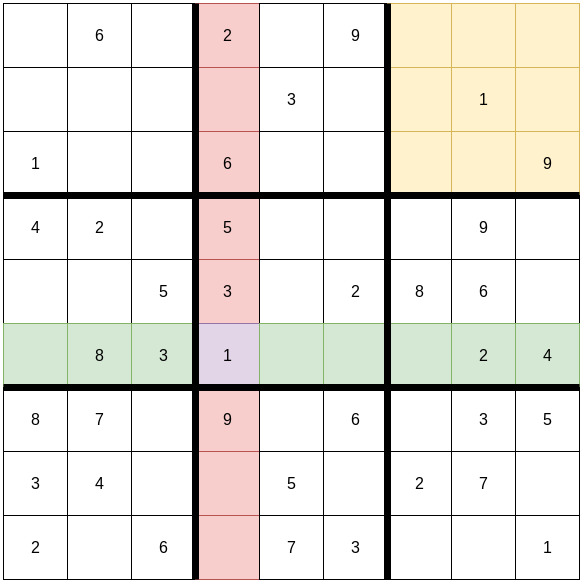
\includegraphics[width=\textwidth]{Pictures/Leer.png}
        \end{column}
        \begin{column}{0.55\textwidth}
            \begin{itemize}
                \item 9x9 Gitter mit Zahlen von 1 bis 9
                \item leere Felder so ausfüllen, dass jede Zahl in
                jeder Zeile, jeder Spalte und jedem 3x3-Block genau 1-mal vorkommt
                \item verschiedene Schwierigkeitsgrade in Abhängigkeit von Anzahl 
                gegebener Felder
                \item weitere Varianten wie z.B. 25x25
                \item BruteForce: \(9^{41}=1.3\cdot 10^{39}\) - \(9^{64}=1,2\cdot 10^{61}\) Möglichkeiten (abhängig von Schwierigkeit)
            \end{itemize}
        \end{column}
    \end{columns}
\end{frame}
\begin{frame}{Kodierung}
    \begin{columns}[T] % T aligns the tops of the columns
        \begin{column}{0.75\textwidth}
            \includegraphics[width=\textwidth]{Pictures/Repräsentation.png}
        \end{column}
        \begin{column}{0.35\textwidth}
            \begin{itemize}
                \item Verwendung von shared\_ptr
                \item leere Felder \(=0\)
                \item Reihenrepräsentation \(\rightarrow\) 1D-Array
                \item Gitterrepräsentation \(\rightarrow\) 2D-Array
            \end{itemize}
        \end{column}
    \end{columns}
    \note[item]{2 Repraesentationen}
    \note[item]{aenderung in einer -> aenderung in anderer}
\end{frame}

\begin{frame}{Initialisierung}
    \begin{columns}[T] % T aligns the tops of the columns
        \begin{column}{0.75\textwidth}
            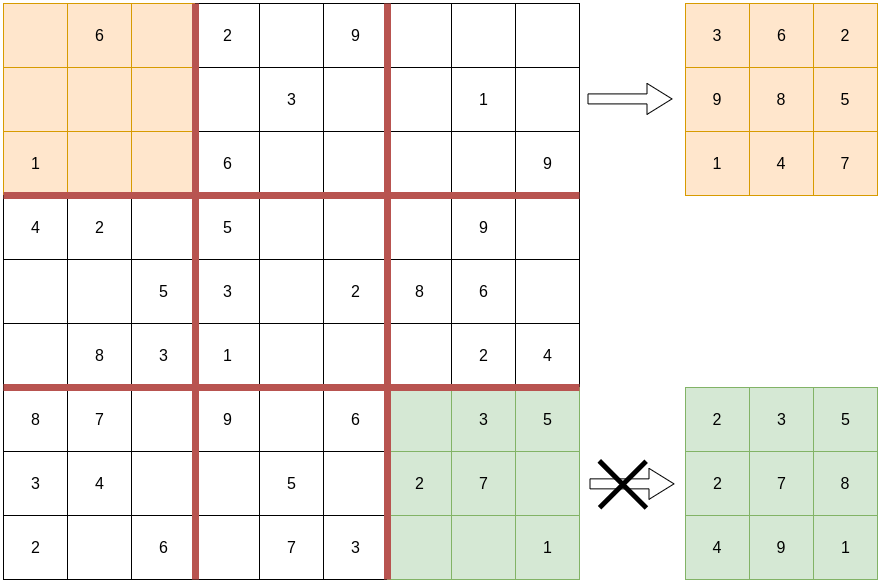
\includegraphics[width=\textwidth]{Pictures/Initialisierung.png}
        \end{column}
        \begin{column}{0.35\textwidth}
            \begin{itemize}
                \item zufällige Initialisierung leerer Felder
                \item einfache Methode: keine doppelten in Blöcken
                \item intelligente Initialisierung: möglichst keine doppelten in Zeilen
            \end{itemize}
        \end{column}
    \end{columns}
\end{frame}

\section{Fitnessfunktion}
\begin{frame}{Fitnessberechnung}
    \begin{columns}[T] % T aligns the tops of the columns
        \begin{column}{0.75\textwidth}
            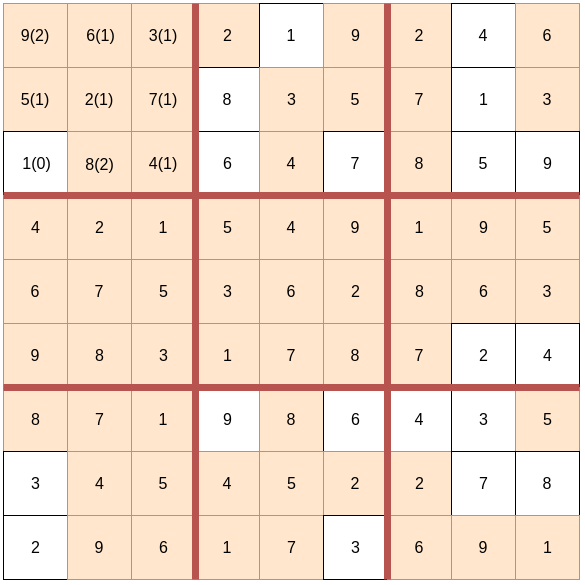
\includegraphics[width=\textwidth]{Pictures/Collision-Fitness.png}
        \end{column}
        \begin{column}{0.35\textwidth}
            \begin{itemize}
                \item Kollisionszahl als Fitnesswert (=86)
                \item Speicherung individueller Werte für Zellen \\
                (s. Block 0)
            \end{itemize}
            Andere Idee für Fitnessberechnung:
            \begin{itemize}
                \item \(|\sum_{i=0}^{9}i-\sum_{i=0}^{9}x_{ij}|\) (Zeile0 \(\rightarrow\) 3)
                \item \(|9!-\prod_{i=0}^{9}x_{ij}|\) (Zeile0 \(\rightarrow\) 222912)
                \item \(|\{1,2,...,9\}\setminus \{x_{0j},x_{1j},...,x_{8j}\}|\) (Zeile0 \(\rightarrow\) 3)
            \end{itemize}
        \end{column}
    \end{columns}
\end{frame}

\begin{frame}{Selektion}
    \begin{columns}[T] % T aligns the tops of the columns
        \begin{column}{0.4\textwidth}
            \textbf{Elitismus:}
            \newline
            \begin{itemize}
                \item Wahl der besten x-Prozent der Individuen
                \item Vorteil: schnelles Erreichen des (lokalen) Minimums
                \item Nachteil: eventuell globales Minimum schwerer zu erreichen
            \end{itemize}
        \end{column}
        \begin{column}{0.6\textwidth}
            \textbf{Glücksradauswahl (universelles Stichprobenziehen):}
            \begin{itemize}
                \item Skalierung der Fitness, sodass die Summe der
                Fitnesswerte 1 ergibt
                \item hintereinander reihen der Individuen mit ihren Fitnesswerten
                \item Auswahl von Individuen in gleichmäßigen Abständen (angepasst an Selektionsrate)
                \item Vorteil: höhere Diversität
                \item Nachteil: langsamere Konvergenz
            \end{itemize}
        \end{column}
    \end{columns}
\end{frame}
\begin{frame}{Mutation}
    \begin{columns}[T] % T aligns the tops of the columns
        \begin{column}{0.75\textwidth}
            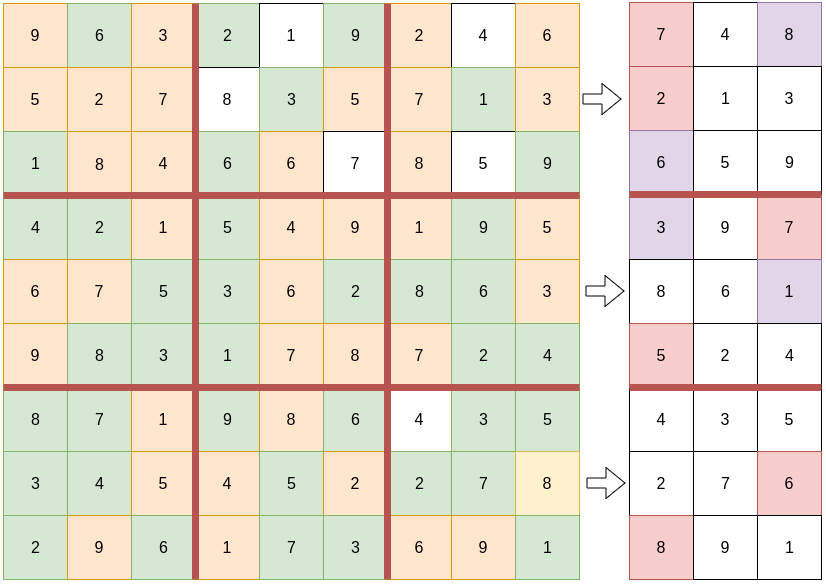
\includegraphics[width=\textwidth]{Pictures/Mutation.png}
        \end{column}
        \begin{column}{0.35\textwidth}
            \begin{itemize}
                \item Ausführung blockweise
                \item gegebene Felder werden ignoriert
            \end{itemize}
            \begin{enumerate}
                \item Auswählen von Kollisionszellen (beliebige Chance für andere Zellen) 
                \item zufälliges paarweises Austauschen der gewählten Zellen
            \end{enumerate}
        \end{column}
    \end{columns}
    \note[item]{grid-repraesentation und Fitness-Sudoku benoetigt}
    \note[item]{blockweise ausgefuehrt}
    \note[item]{gruen bleibt, rot tauschen, weiss Wahrscheinlichkeits tausch}
    \note[item]{--> Feld mit 1 Kollision kann trotzdem noch tauschen}
    \note[item]{weniger Minima -> groessere Exploration}
    \note[item]{Liste aller Zahlen}
    \note[item]{Zufaelliges Auswaehlen von Tauschpaaren}
    \note[item]{uebrige zurueckschreiben}
\end{frame}

\begin{frame}{2-Punkt-Crossover}
    \centering
    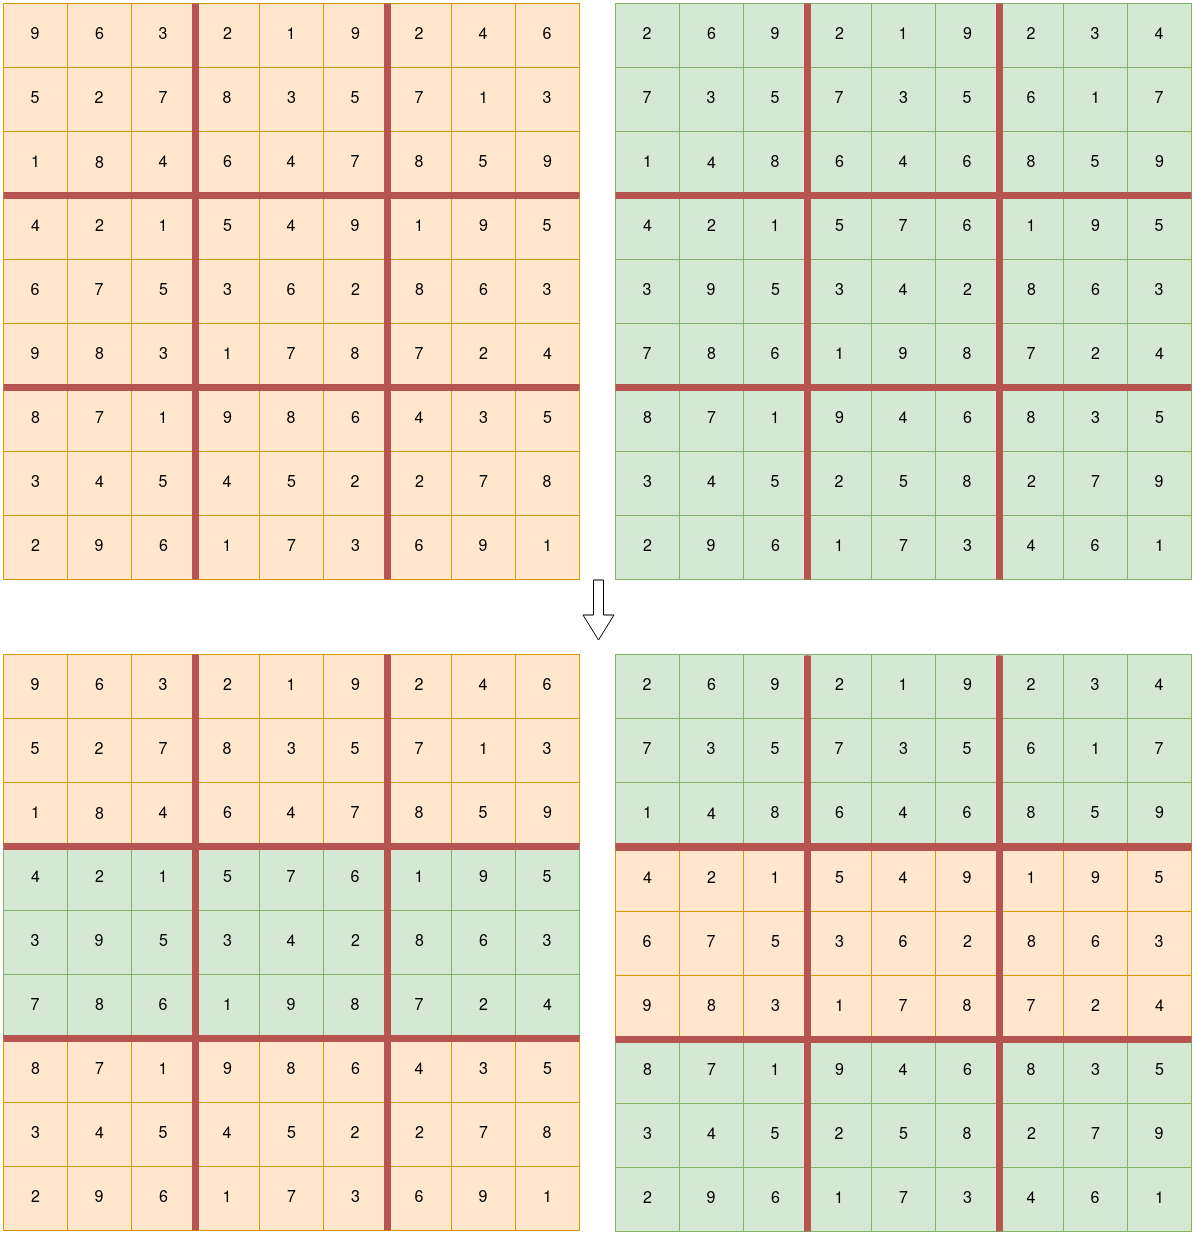
\includegraphics[width=0.7\textwidth]{Pictures/2-Punkt-Crossover.png}
\end{frame}
\begin{frame}{Diagonales-Crossover}
    \centering
    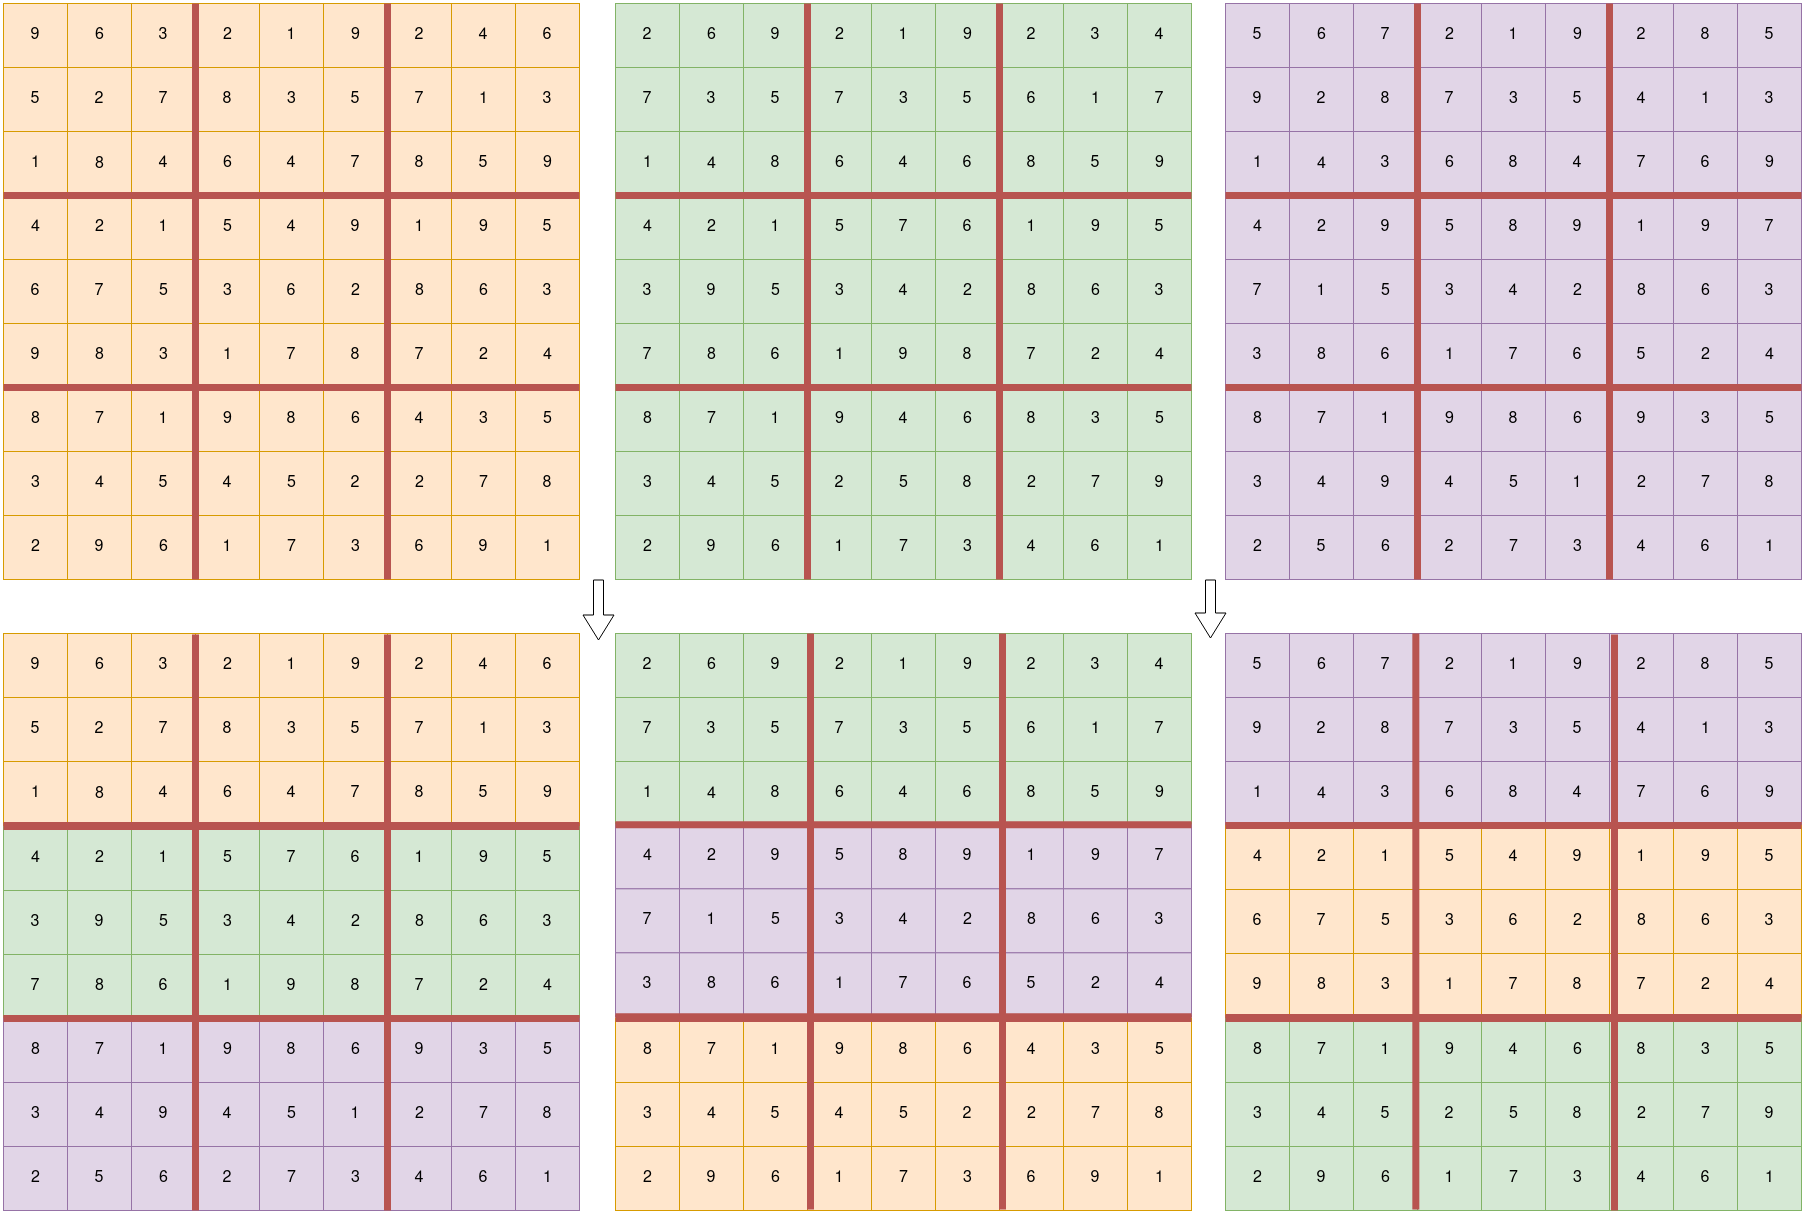
\includegraphics[width=\textwidth]{Pictures/Diagonales-Crossover.png}
\end{frame}
\begin{frame}{Zusammensetzung}
    beste Zusammensetzung (empirisch):
    \begin{enumerate}
        \item Standard-Initialisierung (effizienter)
        \item Fitnessberechnung
        \item Selektion (20\%)
        \item Mutation (\(\frac{1}{9}\) \- Wahrscheinlichkeit für nicht kollidierende Felder)
        \item diagonales Crossover (größere Diversität)
    \end{enumerate}
    Abbruchkriterium: 25 Generation ohne Verbesserung des Fitnesswertes
    \note[item]{Testen: oft lokales Minimum}
    \note[item]{Ziel: moeglichst viel Exploration und trotzdem noch konvergenz}
    \note[item]{punish_same ohne Erfolg}
    \note[item]{Initialisierung: Standard (zwar initial schlechter, aber mehr Exploration) + effizienter}
    \note[item]{Fitness: nur 1 Variante}
    \note[item]{Selektion: universelles Stichprobenziehen konvergiert fast garnicht}
    \note[item]{20\% Elitismus als bester empirische Wert}
    \note[item]{Crossover: diagonal --> mehr Diversitaet}
    \note[item]{Abbruch: 25 Gen. (empirisch ist da bester Wert = Durchschnitt)}
\end{frame}
\begin{frame}{Auswertung}
    Test auf 40 Sudokus (10 aus jeder Schwierigkeitsstufe 
    (Leicht, Mittel, Schwer, Extrem)):
    \newline
    \newline
    \textbf{Populationsgröße 100:}
    \newline
    \newline
    \scalebox{0.7}{
        \begin{tabular}[width=0.7\textwidth]{c|c|c|c|c}
            Schwierigkeit & gelöst (\%) & durchschnittliche & durchschnittliche & durchschnittliche  \\
            & & Zeit (ms) & Generationen & Zeit(Abbruch) (ms)\\
            \hline
            Leicht & 100 & 1102 & 7.2 & - \\
            Mittel & 60 & 2721 & 18.8 & 6381 \\
            Schwer & 0 & - & 32.3 & 9412 \\
            Experte & 0 & - & 33.4 & 9583 \\
        \end{tabular}
    }
    \newline
    \newline
    \newline
    \textbf{Populationsgröße 500:}
    \newline
    \newline
    \scalebox{0.7}{
        \begin{tabular}{c|c|c|c|c}
            Schwierigkeit & gelöst (\%) & durchschnittliche & durchschnittliche & durchschnittliche  \\
             & & Zeit (ms) & Generationen & Zeit(Abbruch) (ms)\\
            \hline
            Leicht & 100 & 4662 & 5.6 & - \\
            Mittel & 90 & 13222 & 11 & 35048 \\
            Schwer & 50 & 25979 & 32,4 & 53385 \\
            Experte & 0 & - & 40.1 & 51216 \\
        \end{tabular}
    }
\end{frame}
\begin{frame}{Auswertung}
    \textbf{Populationsgröße 1000:}
    \newline
    \newline
    \scalebox{0.7}{
    \begin{tabular}{c|c|c|c|c}
        Schwierigkeit & gelöst (\%) & durchschnittliche & durchschnittliche & durchschnittliche  \\
         & & Zeit (ms) & Generationen & Zeit(Abbruch) (ms)\\
        \hline
        Leicht & 100 & 9208 & 5.3 & - \\
        Mittel & 100 & 24384 & 14.8 & - \\
        Schwer & 60 & 43039 & 25.5 & 87460 \\
        Experte & 20 & 91698 & 54,5 & 123294 \\
    \end{tabular}
    }
\end{frame}
\begin{frame}{Ausblick}
    \begin{columns}[T] % T aligns the tops of the columns
        \begin{column}{0.3\textwidth}
            \vspace*{0.5cm}
            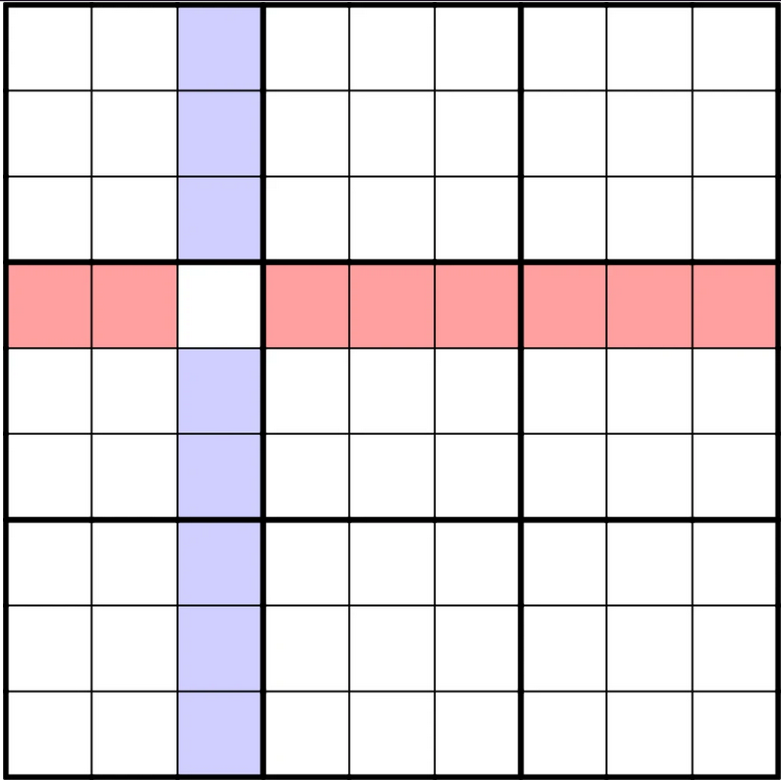
\includegraphics[width=\textwidth]{Pictures/H3.png} \\
            \vspace*{0.5cm}
            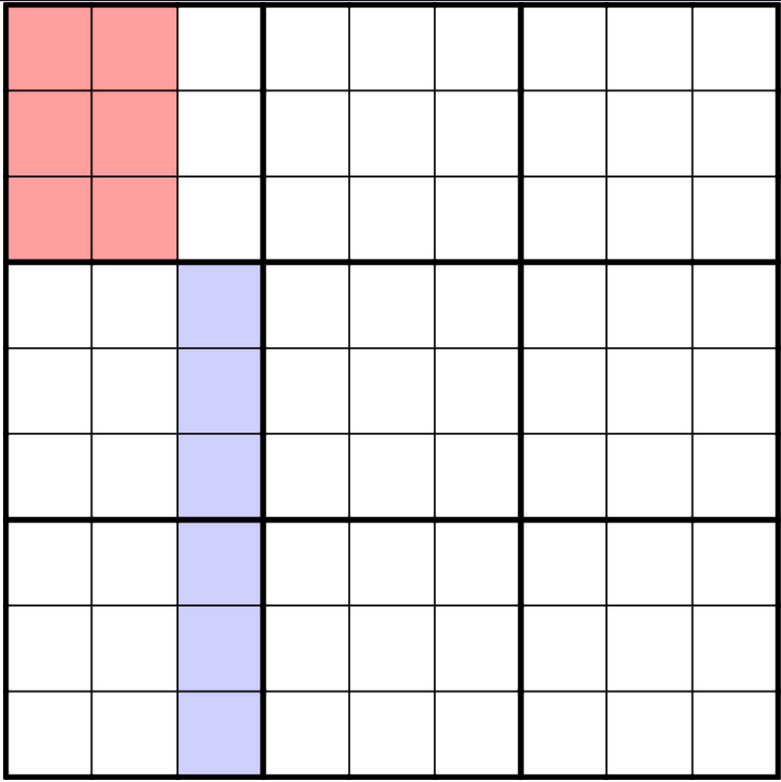
\includegraphics[width=\textwidth]{Pictures/H5.png}
        \end{column}
        \begin{column}{0.3\textwidth}
            \vspace*{0.5cm}
            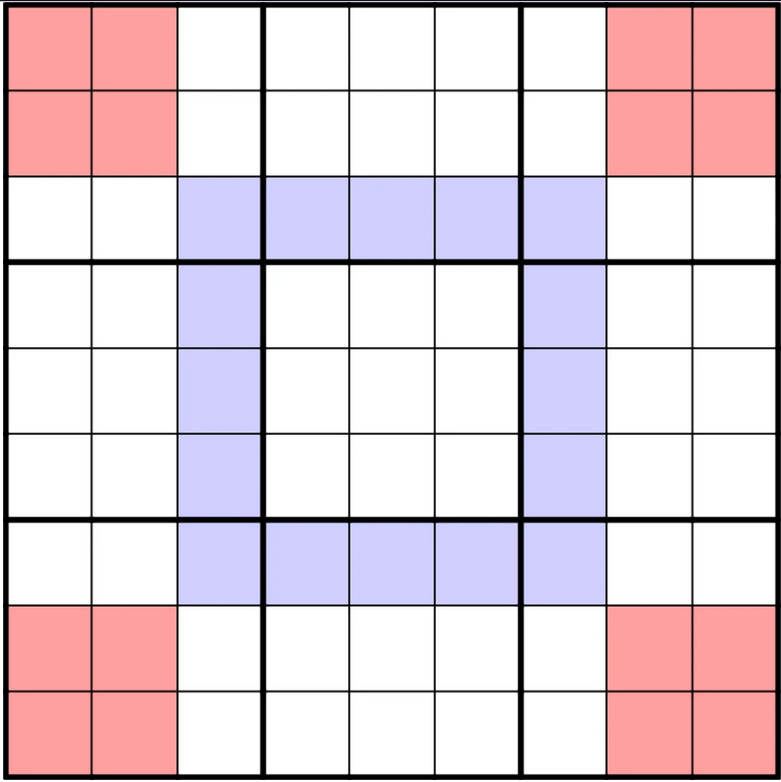
\includegraphics[width=\textwidth]{Pictures/H1.png} \\
            \vspace*{0.5cm}
            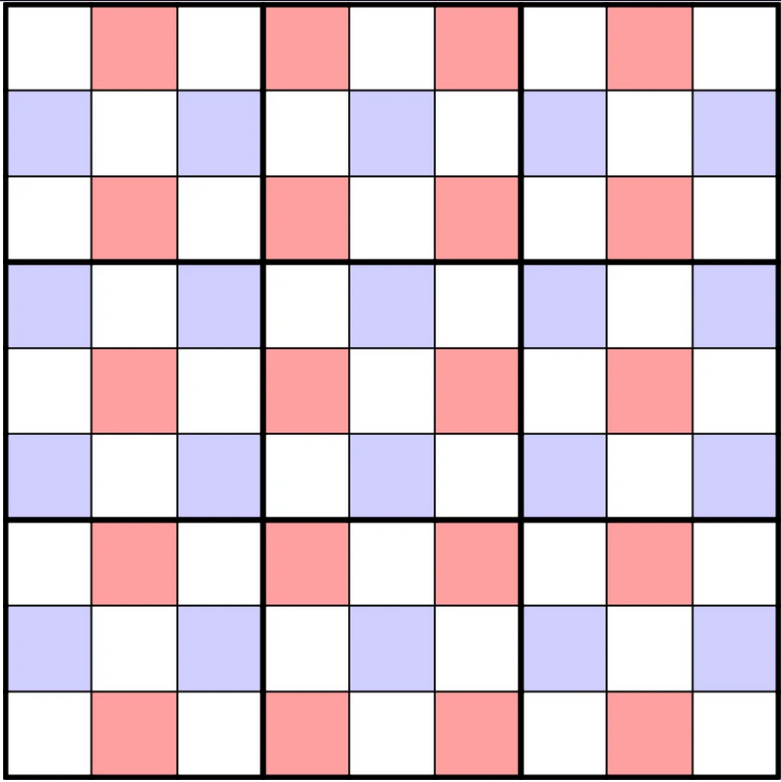
\includegraphics[width=\textwidth]{Pictures/H4.png}
            \cite{SET}
        \end{column}
        \begin{column}{0.35\textwidth}
            \vspace*{0.5cm}
            \begin{itemize}
                \item Anwenden von Set AEquivalenz Theorie (z.B. in Fitnessbewertung oder Mutation)
                \item mehr Exploration durch andere Selektionsverfahren
                \item Anpassung an andere Sudokuarten
            \end{itemize}
        \end{column}
    \end{columns}
    \note[item]{Anwenden von Set Aequivalenz Theorie (z.B. in Fitnessbewertung)}
    \note[item]{eventuell flexiblerer Selektionsdruck (um zu Beginn mehr Exploration zu haben)}
    \note[item]{Anpassung an andere Sudokuarten, z.B. Freiform Sudoku oder groessere Arten}
    \note[item]{GUI-Erklaeren}
\end{frame}
\section{Vorführung}
\begin{frame}{Quellen}
  \bibliography{Ausarbeitung/bibliography.bib}
  \bibliographystyle{abbrv}
\end{frame}
\end{document}